\documentclass[12pt,oneside,notitlepage,titleauthor]{mwart}%draft
\usepackage[utf8]{inputenc}
\usepackage{polski}
\usepackage[T1]{fontenc} 
\linespread{1.3}
\usepackage{geometry,graphicx,url}
%\usepackage{fancyhdr,graphics,geometry,array,multicol,longtable,tabularx,color,graphicx,rotating,url}
\geometry{a4paper,top=2.5cm,bottom=2.5cm,left=3.5cm,right=2.5cm}

\urldef\grant\url{https://bitbucket.org/jsbien/ndt}
\title{Przeglądarka materiałów leksykograficznych \texttt{Maleks}. \\Podręcznik użytkownika}%\thanks{Test \grant}}
\author{Joanna Bilińska\\Katedra Lingwistyki Formalnej UW}
\date{maj 2012 r.}
\begin{document}
\maketitle

\begin{quotation}
Opisywany program i niniejsza dokumentacja zostały sfinansowane przez grant \textit{Narzędzia dygitalizacji tekstów na potrzeby badań filologicznych} --- grant MNiSzW nr NN519 384036 (\url{https://bitbucket.org/jsbien/ndt}) kierowany przez Janusza S. Bienia. 

W dokumentacji (i eksperymentach) wykorzystano próbkę około 10~000 skanów fiszek kartoteki \textit{Słownika języka polskiego XVII i 1. połowy XVIII wieku}  (\url{http://sxvii.pl}).
\end{quotation}

\section{O programie}


Przeglądarka materiałów leksykograficznych \texttt{maleks} została przygotowana w Katedrze Lingwistyki Formalnej UW przez Tomasza Olejniczaka\footnote{\url{https://bitbucket.org/tomek87/maleks}}   według specyfikacji Janusza S. Bienia. Założenia zostały przedstawione w tekście Janusza S. Bienia pt.~\textit{Dygitalizacja kartotek słownikowych} (w druku)\footnote{\url{http://bc.klf.uw.edu.pl/256/}}.

Program ten służy do przeglądania i indeksowania przede wszystkim zeskanowanych fiszek, np. słownikowych. Mógłby być także wykorzystywany do pracy z~bibliotecznymi kartami katalogowymi.

\texttt{Maleks} współpracuje z bazami danych na zasadzie klient--serwer. Kartoteka, z~której korzystają redaktorzy, musi być zamieszczona lokalnie, serwer natomiast może być zdalny. Informacje o sposobie tworzenia kartoteki znajdują się w źródłach programu.


\begin{figure}[h]
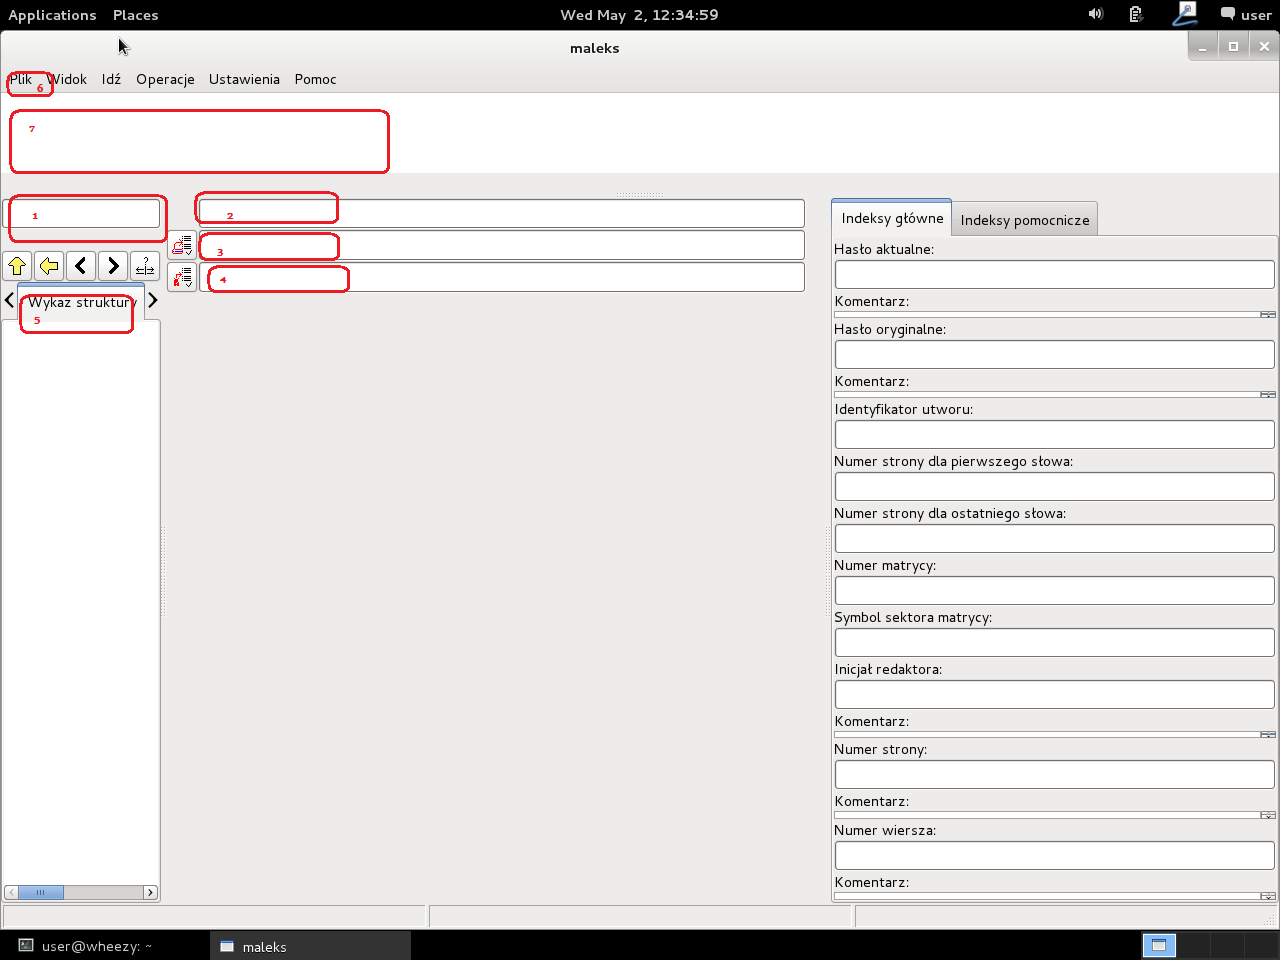
\includegraphics[scale=0.3]{01_puste.png}
\caption{Okno programu \texttt{maleks}}
\label{01_puste}
\end{figure}

Opis podstawowych elementów okna programu (por. rys. \ref{01_puste} na s. \pageref{01_puste}):

\begin{enumerate}
\item pole kwerend,
\item pole hipotez (np. z OCR),
\item pole edycji,
\item pole podpowiedzi (np. z innych słowników),
\item wykazy (tu m.in. wykaz struktury, wykaz haseł),
\item menu programu,
\item pole komunikatów.
\end{enumerate}



\section{Wyszukiwanie}
Aby znaleźć fiszkę, należy w lewym panelu poniżej pola kwerend wybrać \texttt{wykaz haseł}, a następnie w polu kwerend wpisać zapytanie (małymi literami, chyba że listę podpowiedzi mamy z uwzględnieniem wielkich liter) i zatwierdzić ją kombinacją klawiszy \texttt{Ctrl+Enter}. W programie działa tzw. wyszukiwanie przyrostowe (por. rys. \ref{03_wyszukiwanie} na s. \pageref{03_wyszukiwanie}). Oznacza to, że program zaczyna szukać słowa w wykazie haseł już w momencie wpisania pierwszego znaku zapytania, nie czeka na dokończenie wpisywania hasła.  

\begin{figure}[h]
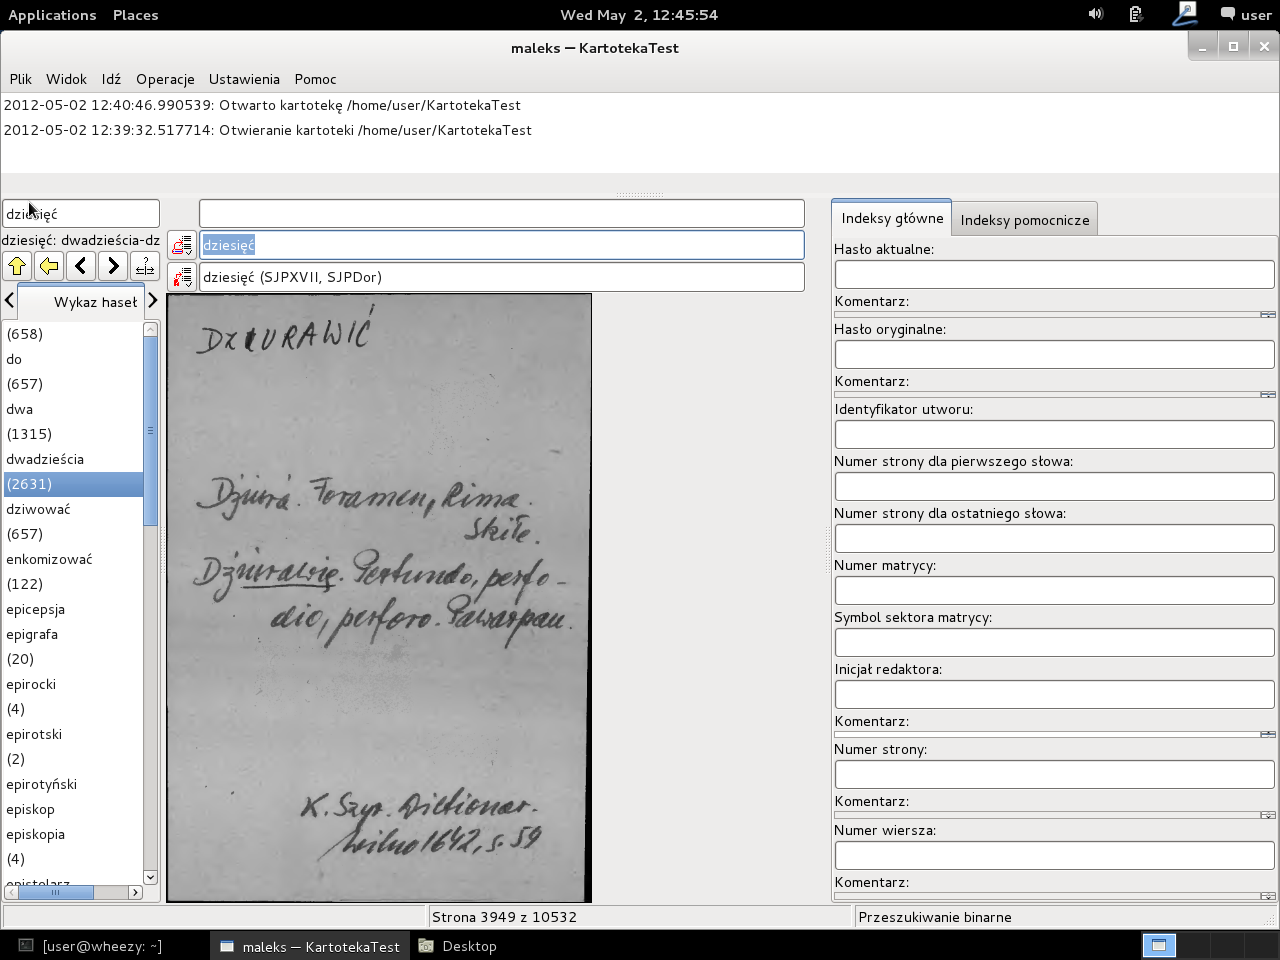
\includegraphics[scale=0.3]{03_wyszukiwanie.png}
\caption{Wyszukiwanie przyrostowe}
\label{03_wyszukiwanie}
\end{figure}
 

W wyniku wyszukiwania program pokaże pierwszą potencjalną fiszkę, a w polu podpowiedzi pojawi się potencjalne hasło (np. z listy haseł w innych słownikach).


\section{Indeksowanie}
Żeby zaindeksować fiszkę (por. rys. \ref{04_indeksowanie} na s. \pageref{04_indeksowanie}), czyli oznaczyć, jakie hasło się na niej znajduje, można w polu edycji (drugi wiersz):

\begin{itemize}
\item zaakceptować podpowiedź z innych słowników (pojawia się w polu podpowiedzi wraz ze wskazaniem, skąd pochodzi) --- w tym celu wpisujemy \texttt{Ctrl+H},
\item zaakceptować odpowiedź z poprzednich indeksowań (pojawia się w polu podpowiedzi) za pomocą skrótu \texttt{Ctrl+H},
\item wpisać hasło samodzielnie, a następnie nacisnąć \texttt{Enter},
\item znaleźć hasło w historii (za pomocą połączenia \texttt{Ctrl} i strzałki), a następnie nacisnąć \texttt{Enter},
\item zaakceptować hasło z pola hipotez, przepisując je do pola edycji i naciskając \texttt{Enter} (por. rys. \ref{ocr} na s. \pageref{ocr}).
\end{itemize}

\begin{figure}[h]
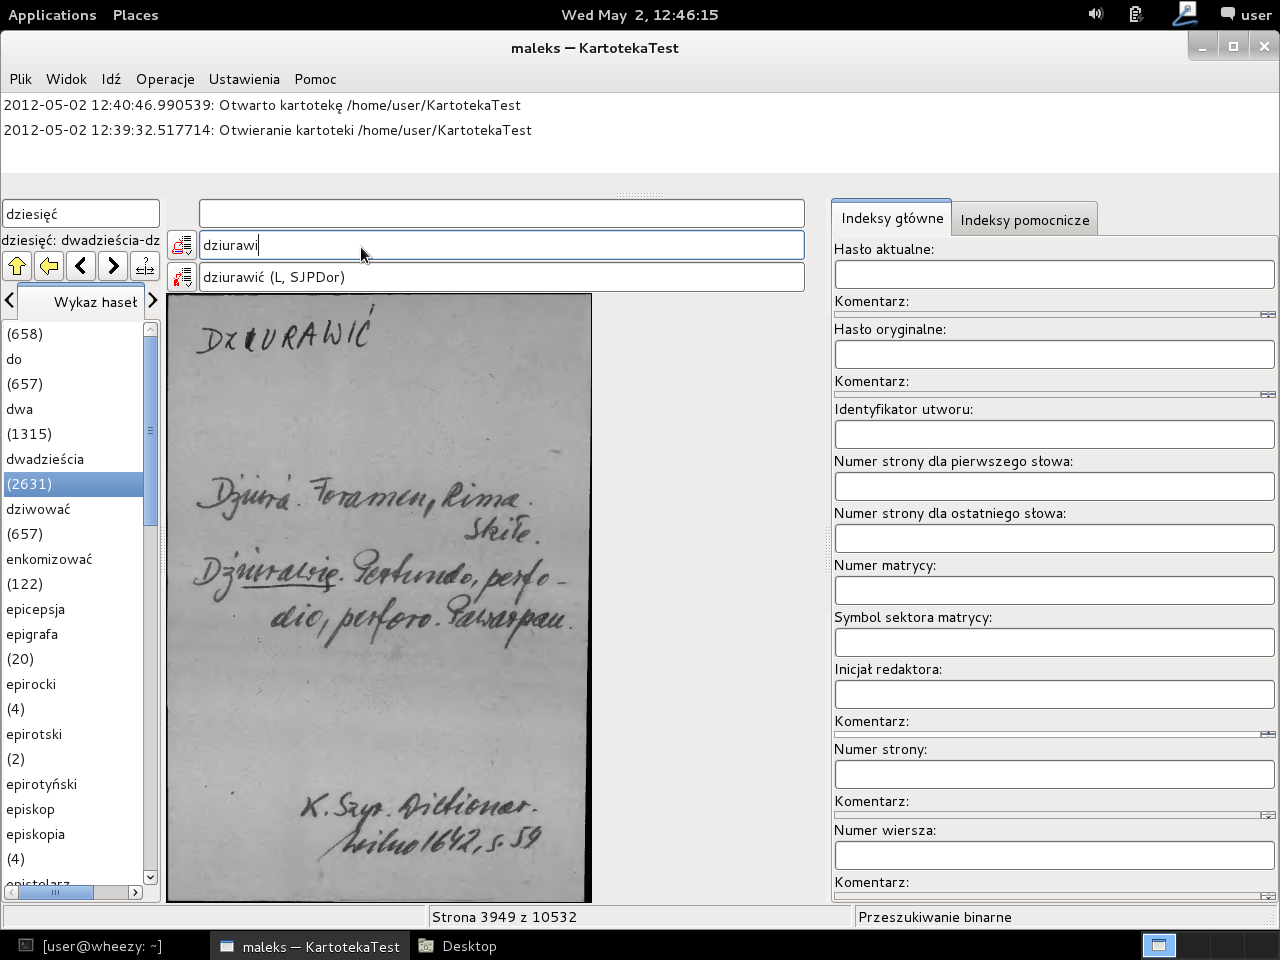
\includegraphics[scale=0.3]{04_indeksowanie.png}
\caption{Indeksowanie}
\label{04_indeksowanie}
\end{figure}


\begin{figure}[h]
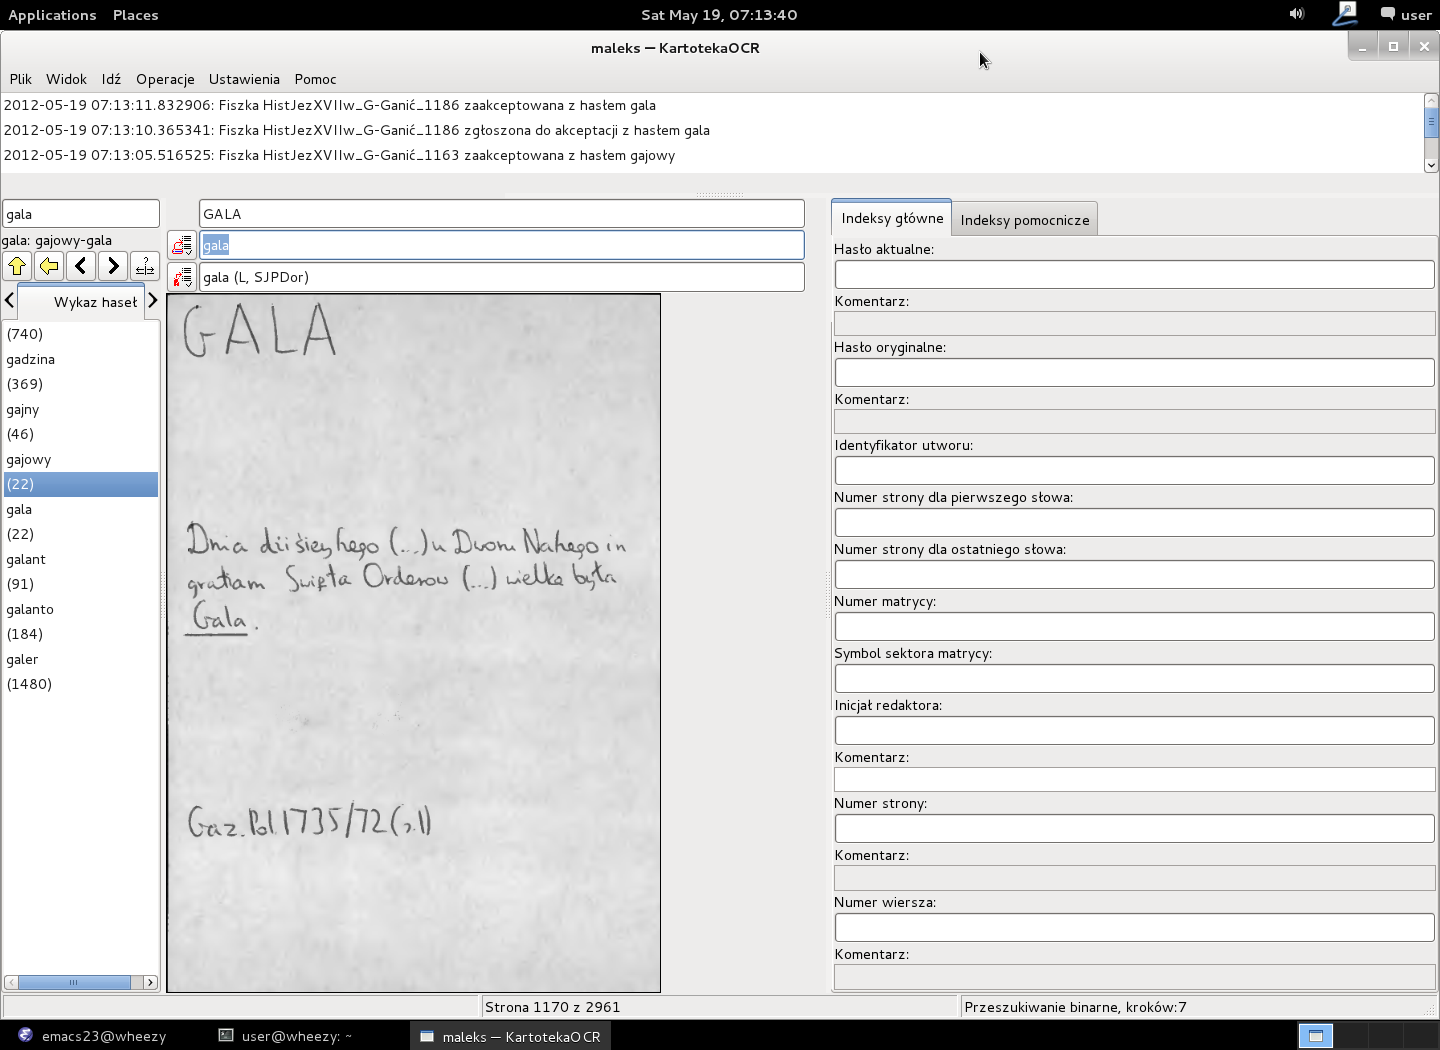
\includegraphics[scale=0.3]{OCR.png}
\caption{Dane z OCR w polu hipotez}
\label{ocr}
\end{figure}

Jeśli użytkownik nie ma pewności co do odczytania informacji z fiszki albo  chce z~innego powodu obejrzeć sąsiednie fiszki, może skorzystać z podglądu. Skrót klawiaturowy \texttt{Ctrl+V} powoduje pojawienie się małego podglądu skanu fiszki (por. rys. \ref{07podglad} na s. \pageref{07podglad}), a za pomocą klawiszy strzałek w górę i w dół można oglądać kolejne i~poprzednie skany.

\begin{figure}[h]
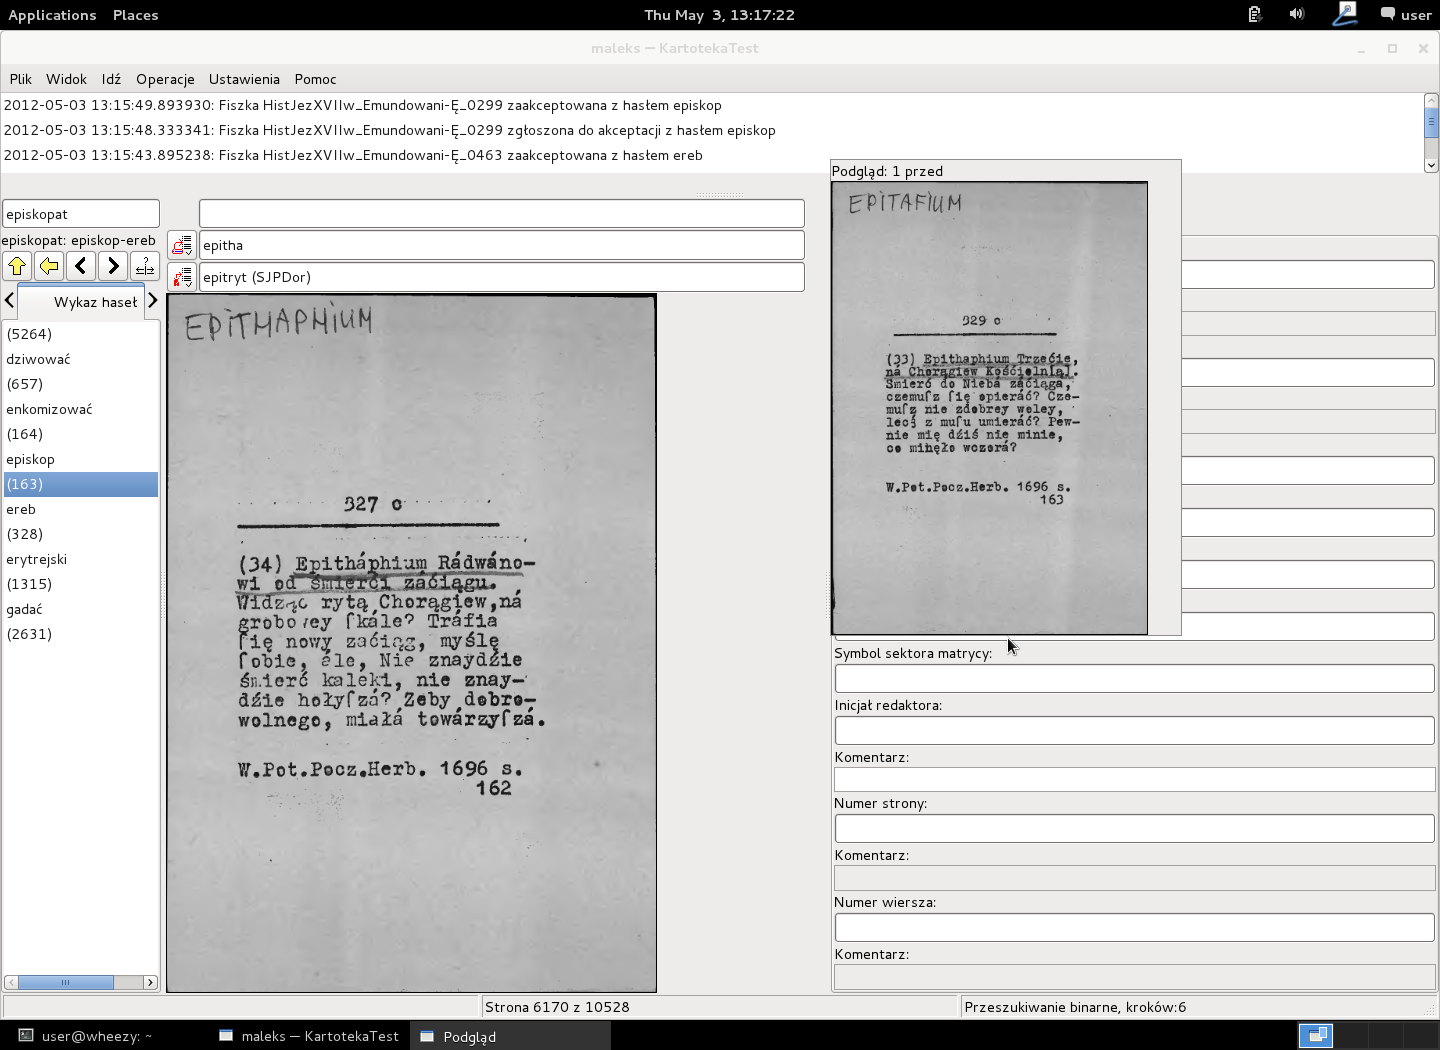
\includegraphics[scale=0.3]{07podglad.png}
\caption{Podgląd fiszki}
\label{07podglad}
\end{figure}

Kiedy hasło zostało znalezione, za pomocą \texttt{Ctrl+Enter} należy wejść w listę hipotetycznych fiszek. Domyślnie nie są one zaindeksowane, mimo że znajdują się w zakresie odpowiadającym naszemu hasłu. Trzeba zaindeksować je ręcznie, korzystając z klawisza \texttt{Enter} dla każdej fiszki (z wskaźnikiem pracy, tzw. fokusem, ustawionym w polu edycji).



\section{Klonowanie fiszek}
Jeśli dana fiszka mogłaby zostać zaindeksowana w dwojaki sposób (np. w dwóch wariantach ortograficznych), można ją sklonować za pomocą skrótu \texttt{Ctrl+K}. Nie działa to jednak w trakcie wyszukiwania binarnego, więc należy je wyłączyć za pomocą skrótu \texttt{Ctrl+B} (po sklonowaniu trzeba wyszukiwanie włączyć ponownie tym samym skrótem).


Podczas klonowania należy określić następujące dane (por. rys. \ref{08klonowanie}  na s. \pageref{08klonowanie}):

\begin{itemize}

\item hasło oryginalne,

\item hasło aktualnej fiszki oryginalnej,

\item hasło aktualnej fiszki sklonowanej.
\end{itemize}

\begin{figure}[h]
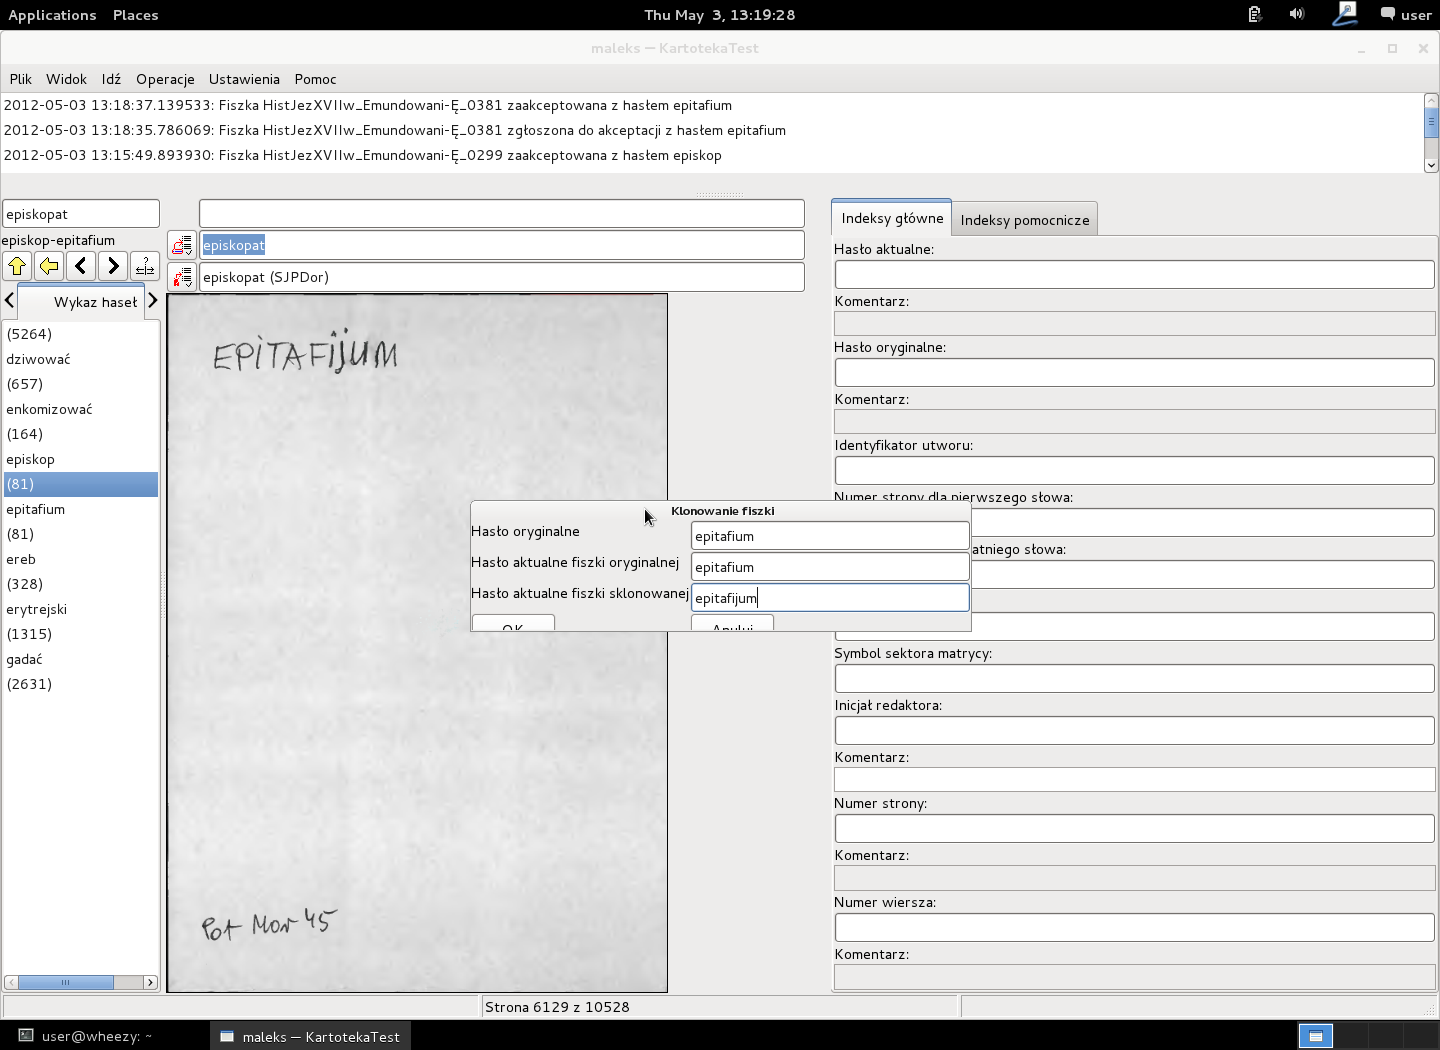
\includegraphics[scale=0.3]{08klonowanie.png}
\caption{Klonowanie fiszki}
\label{08klonowanie}
\end{figure}

\section{Wykaz zadaniowy i zakładki}



Możliwy jest też taki wariant pracy z programem, że użytkownik  sprawdza jedynie zakładki do konkretnych fiszek. Przykładowo redaktor naczelny lub inna osoba wybiera zestaw fiszek, oznacza je zakładkami, a następnie zakładki eksportuje. W ten sposób przygotowuje wykaz zadaniowy, na którym mogą pracować redaktorzy. Przed przystąpieniem do pracy korzysta się wtedy z~opcji \texttt{załaduj wykaz zadaniowy}.

Zakładki do fiszek dodaje się za pomocą skrótu \texttt{Ctrl+D}. Wprawdzie program nie wyświetla żadnego komunikatu o wykonaniu polecenia użytkownika, jednakże poniżej pola kwerend pojawia się lista zakładek (por. rys. \ref{zakladki2} na s. \pageref{zakladki2}). Żeby ją obejrzeć, trzeba zmienić wyświetlanie panelu poniżej pola kwerend z opcji \texttt{wykaz haseł} na \texttt{wykaz zakładek}.

\begin{figure}[h]
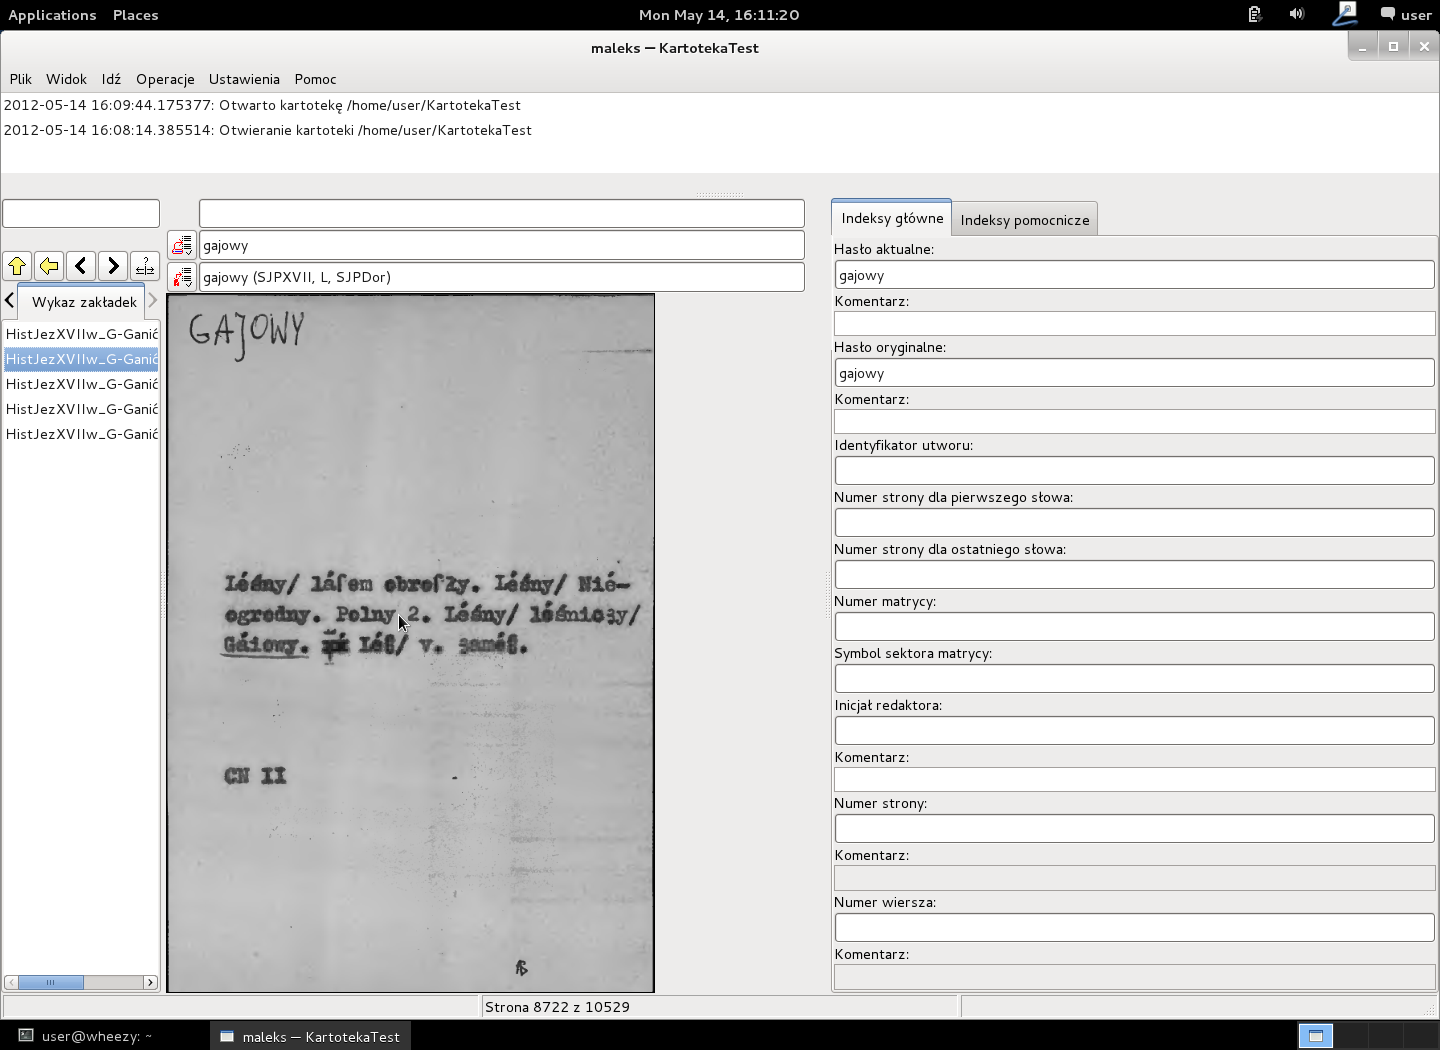
\includegraphics[scale=0.3]{zakladki2.png}
\caption{Zakładki do fiszek}
\label{zakladki2}
\end{figure}

%Serwer dla programu nie musi bowiem znajdować się na tej samej maszynie --- może być np. 1 na pokój. Z programem działają też narzędzia do baz danych.



\section{Przykładowy scenariusz pracy --- indeksowanie okazjonalne}

Otwieramy \texttt{maleks}, a następnie z menu \texttt{Plik} wybieramy \texttt{Ostatnio używane}, a~tam odpowiednią kartotekę. W tym momencie program informuje, że otwiera kartotekę, a po zakończeniu operacji dostajemy komunikat, że kartoteka została otwarta (por. rys. \ref{02_otwartabaza} na s. \pageref{02_otwartabaza}).

\begin{figure}[h]
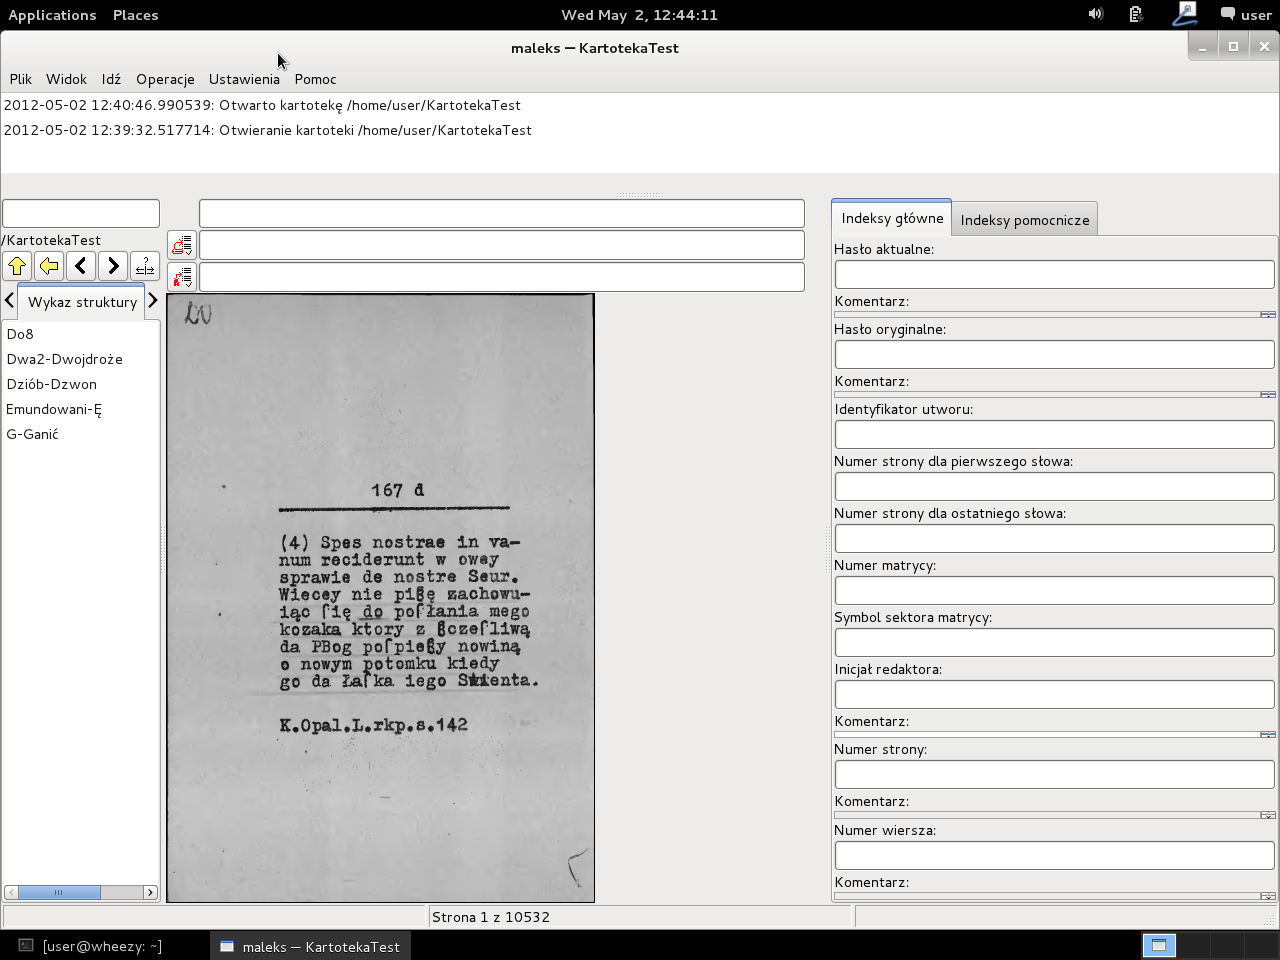
\includegraphics[scale=0.3]{02_otwartabaza.png}
\caption{Otwarta baza}
\label{02_otwartabaza}
\end{figure}

Po otwarciu kartoteki przechodzimy do wykazu haseł i zaczynamy szukać konkretnego hasła, wciskając po wpisaniu \texttt{Enter}.


Program pokazuje hipotetyczną fiszkę wraz z podpowiedziami (por. rys. \ref{01episkopat} na s. \pageref{01episkopat}). 

\begin{figure}[h]
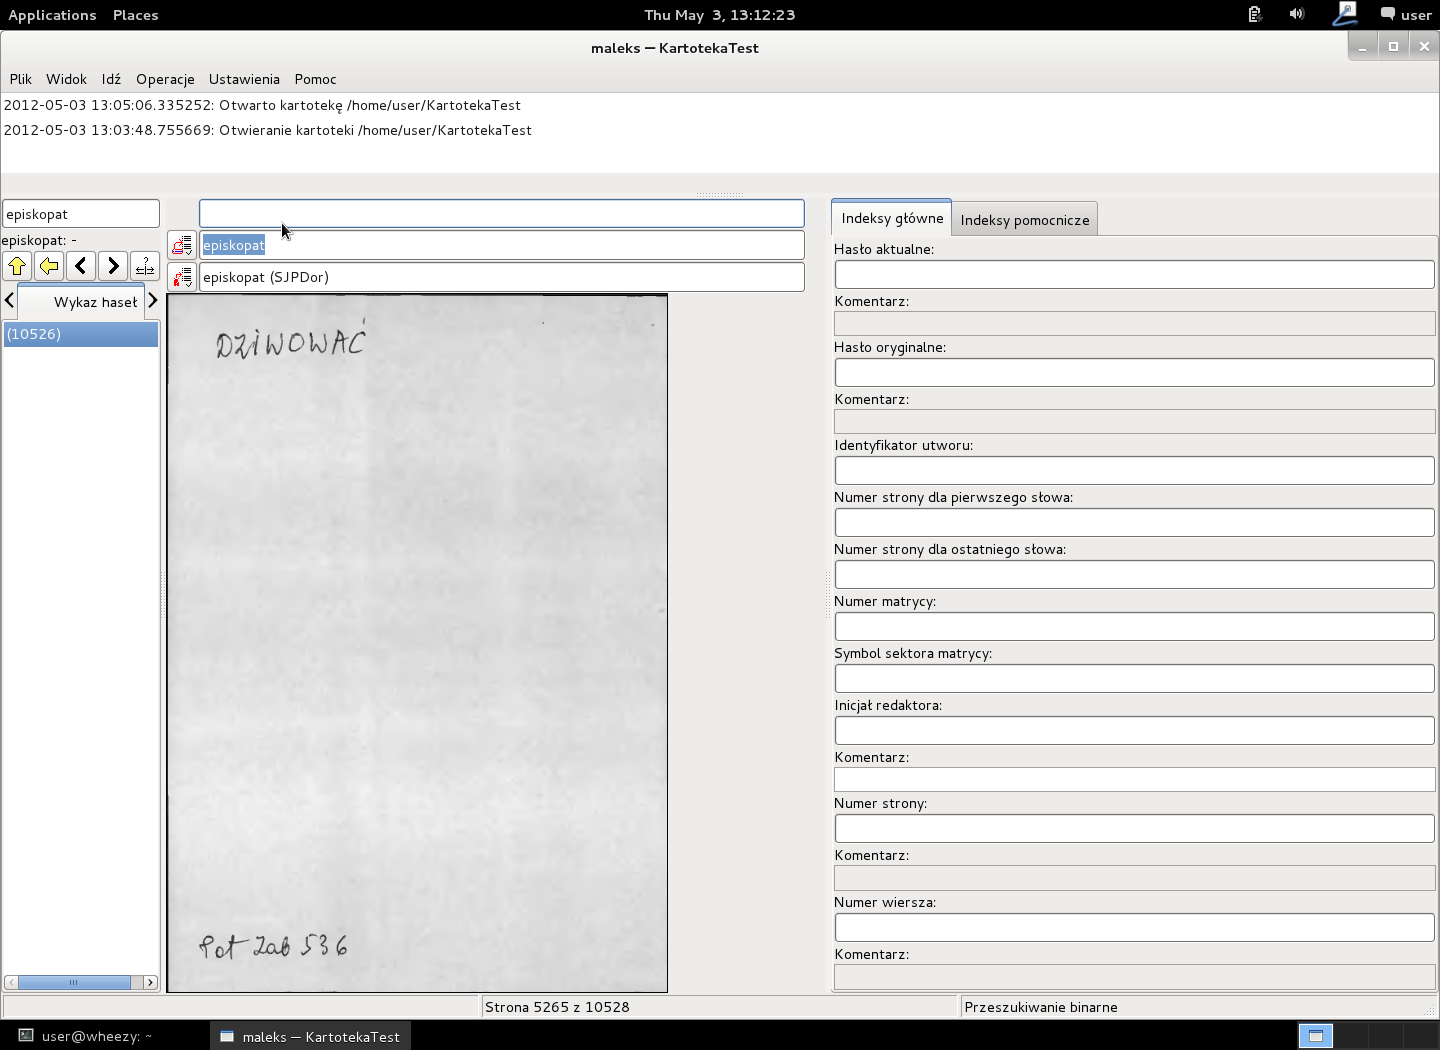
\includegraphics[scale=0.3]{01episkopat.png} 
\caption{Hipotetyczna fiszka}
\label{01episkopat}
\end{figure}

 
Najprawdopodobniej nie jest to szukana przez nas fiszka, więc ją indeksujemy zgodnie z danymi w niej zawartymi, wpisując w górnym polu odpowiednie hasło i~wciskając \texttt{Enter} (por. rys. \ref{02episkopat} na s. \pageref{02episkopat}). 

\begin{figure}[h]
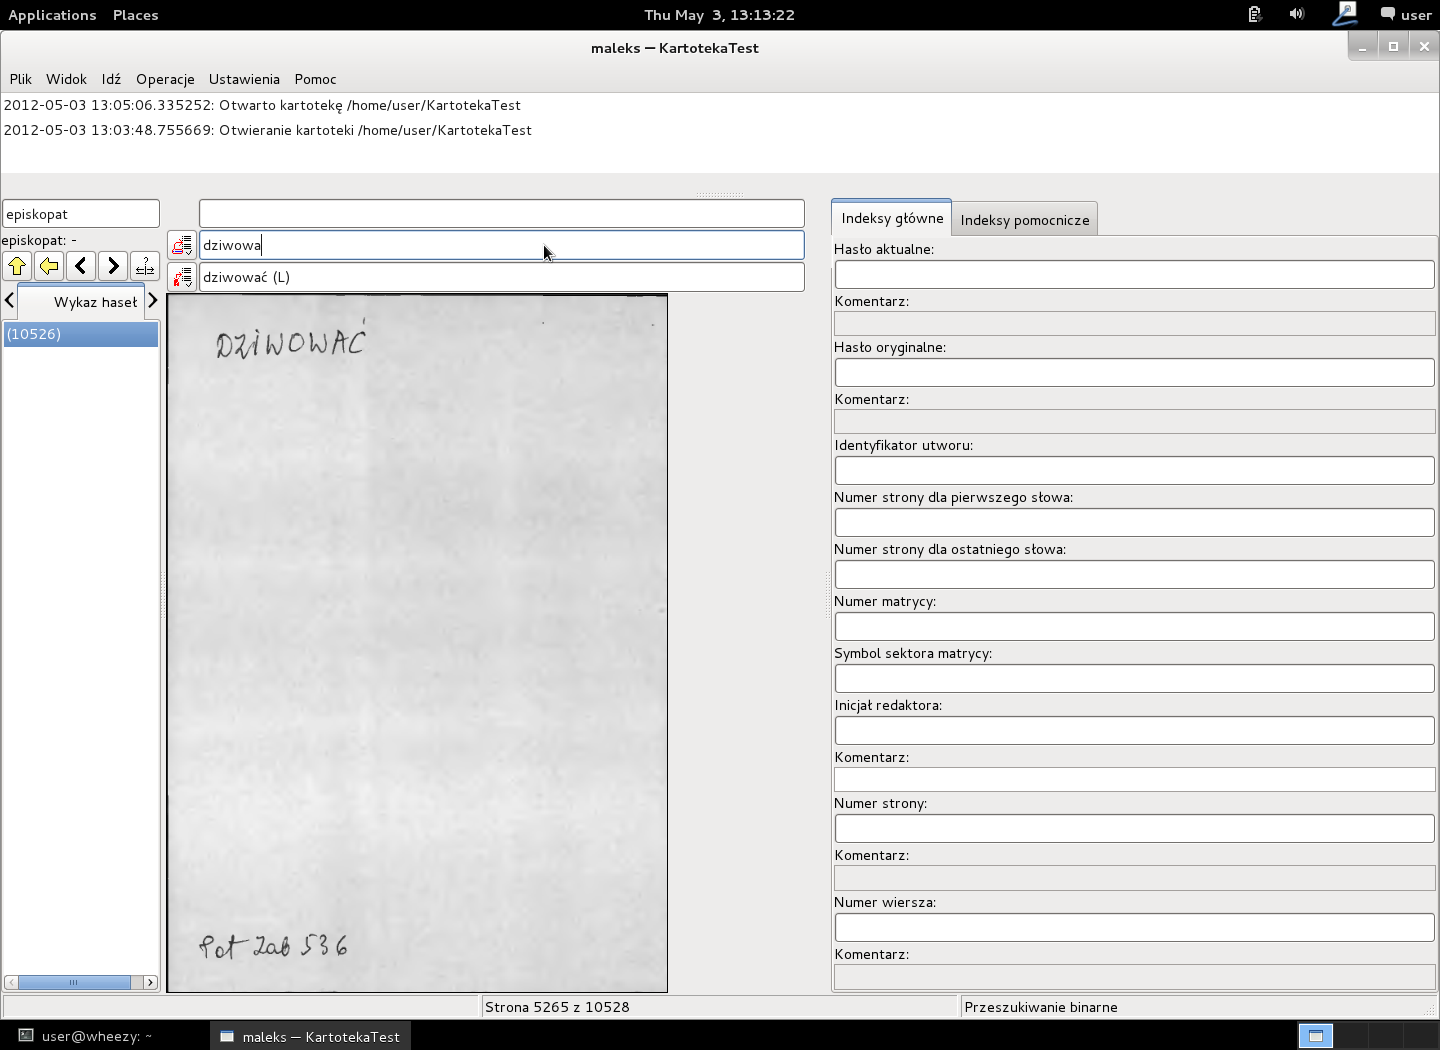
\includegraphics[scale=0.3]{02episkopat.png}
\caption{Indeksowanie}
\label{02episkopat}
\end{figure}

%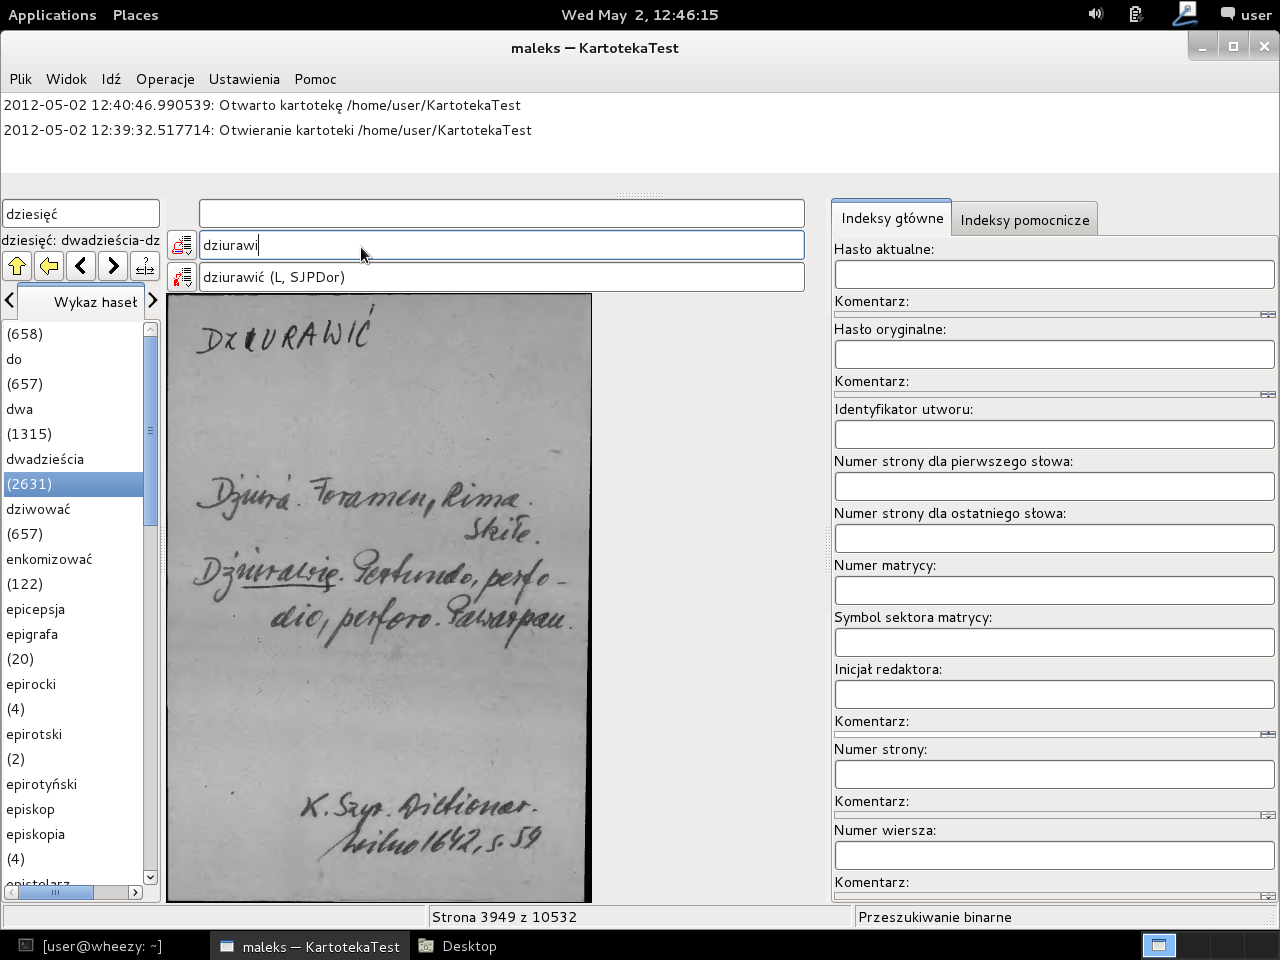
\includegraphics[scale=0.3]{04_indeksowanie.png}

%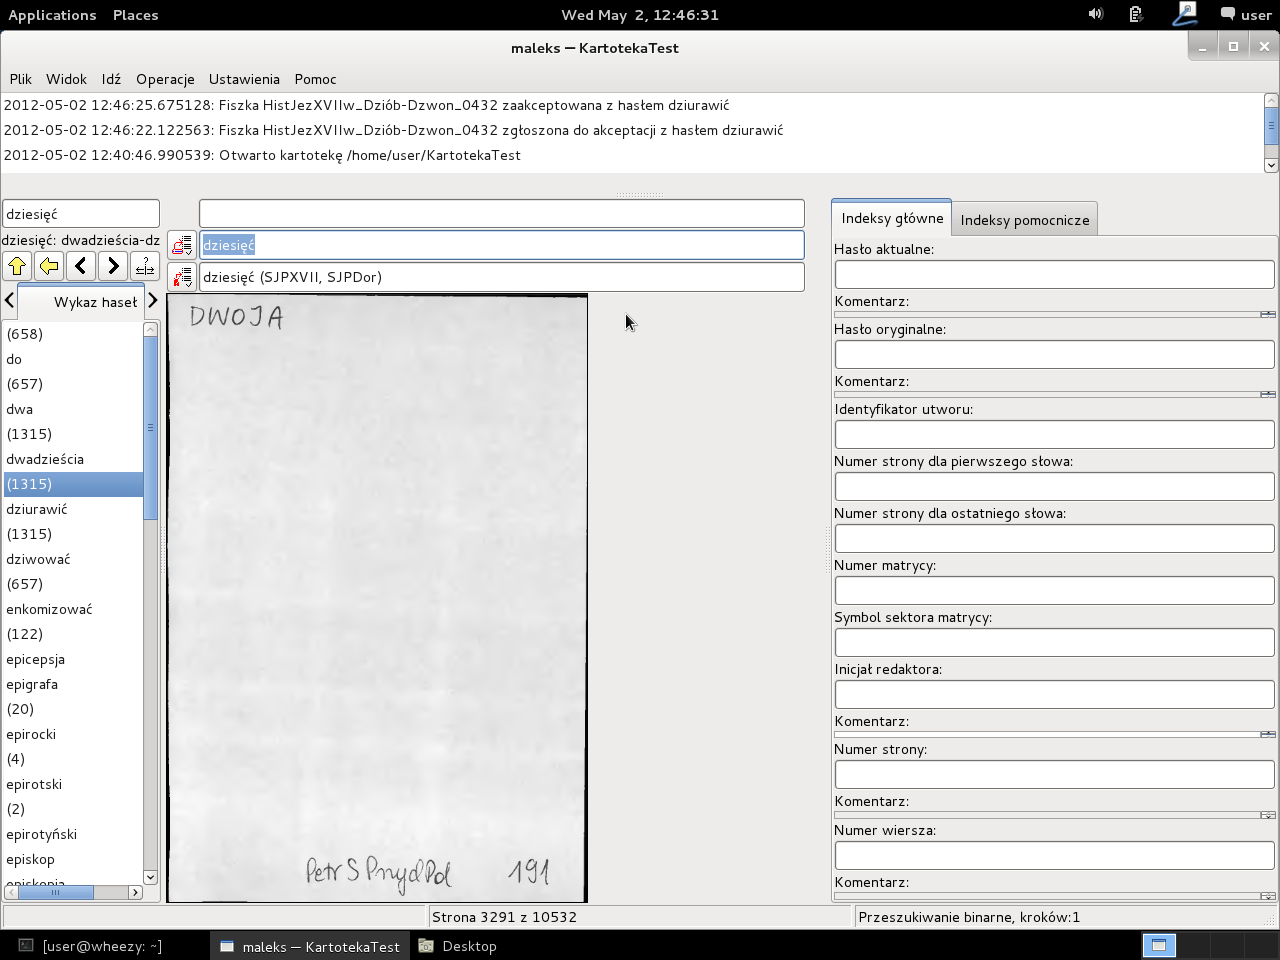
\includegraphics[scale=0.3]{05_indeksowanie2.png}

Program podaje komunikat, że dana fiszka została zaakceptowana z podanym przez nas hasłem (por. rys. \ref{03episkopat} na s. \pageref{03episkopat}.


%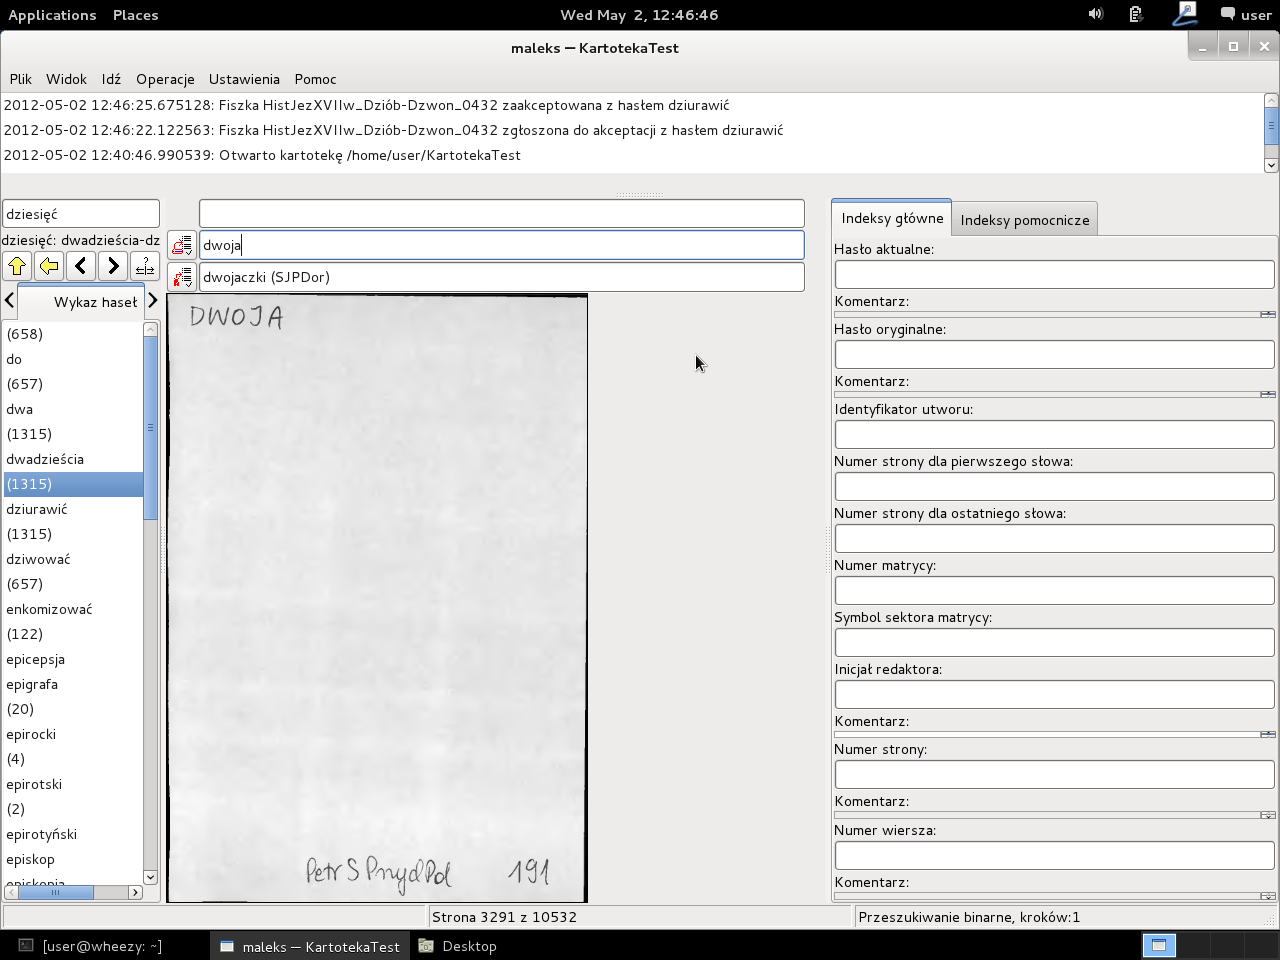
\includegraphics[scale=0.3]{06_indeksowanie3.png}

\begin{figure}[h]
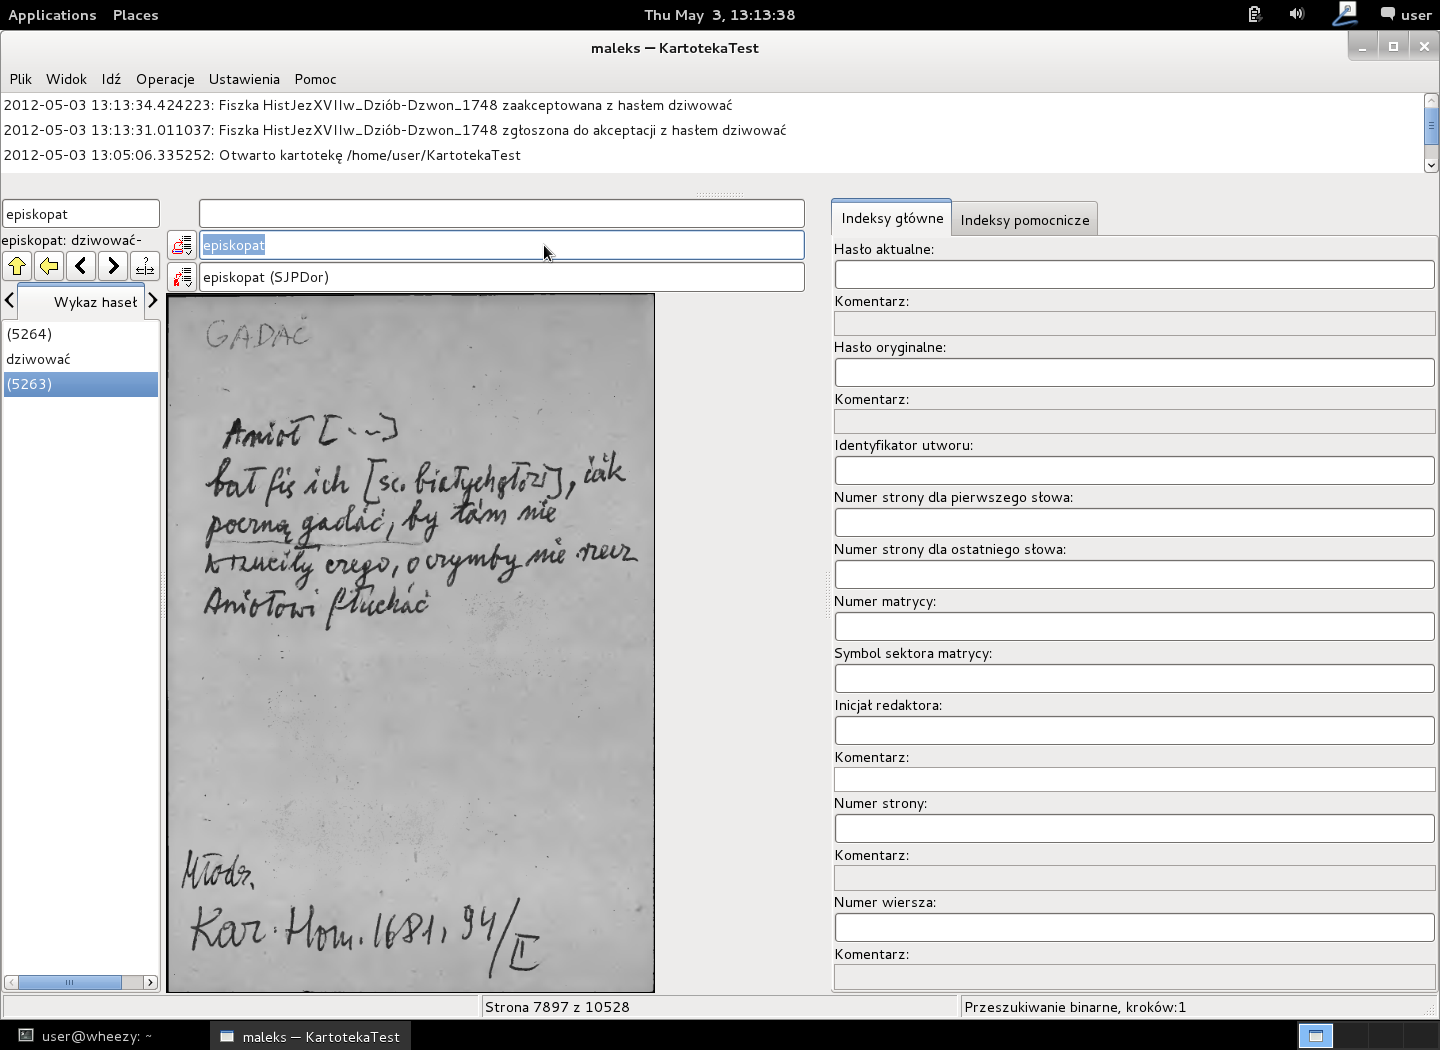
\includegraphics[scale=0.3]{03epispopat.png}
\caption{Komunikat po zaindeksowaniu fiszki}
\label{03episkopat}
\end{figure}

Po zaindeksowaniu przez użytkowania fiszki program kontynuuje wyszukiwanie binarne i~wyświetla kolejną hipotetyczną fiszkę. Zapewne znów nie jest to poszukiwana fiszka, więc indeksujemy ją zgodnie z jej zawartością (por. rys. \ref{binarne} na s. \pageref{binarne}). Jeśli z~jakiegoś powodu wyszukiwanie binarne zostanie wyłączone, można je przywrócić skrótem \texttt{Ctrl+B}.

\begin{figure}[h]
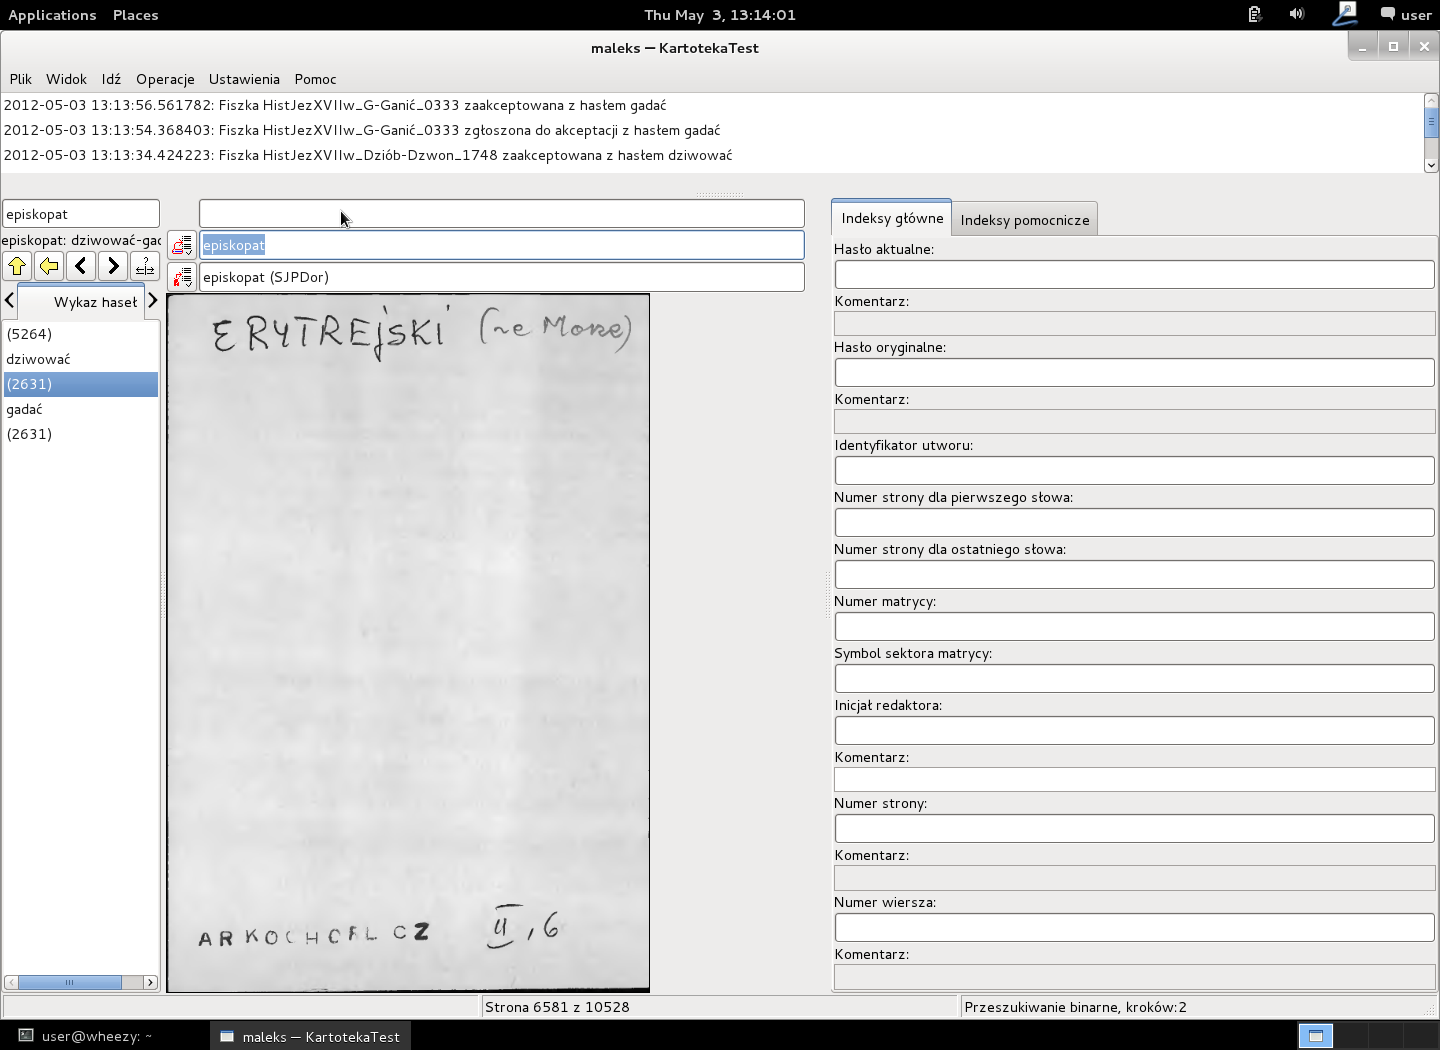
\includegraphics[scale=0.3]{04episkopat_dziura.png}
\caption{Wyszukiwanie binarne}
\label{binarne}
\end{figure}

%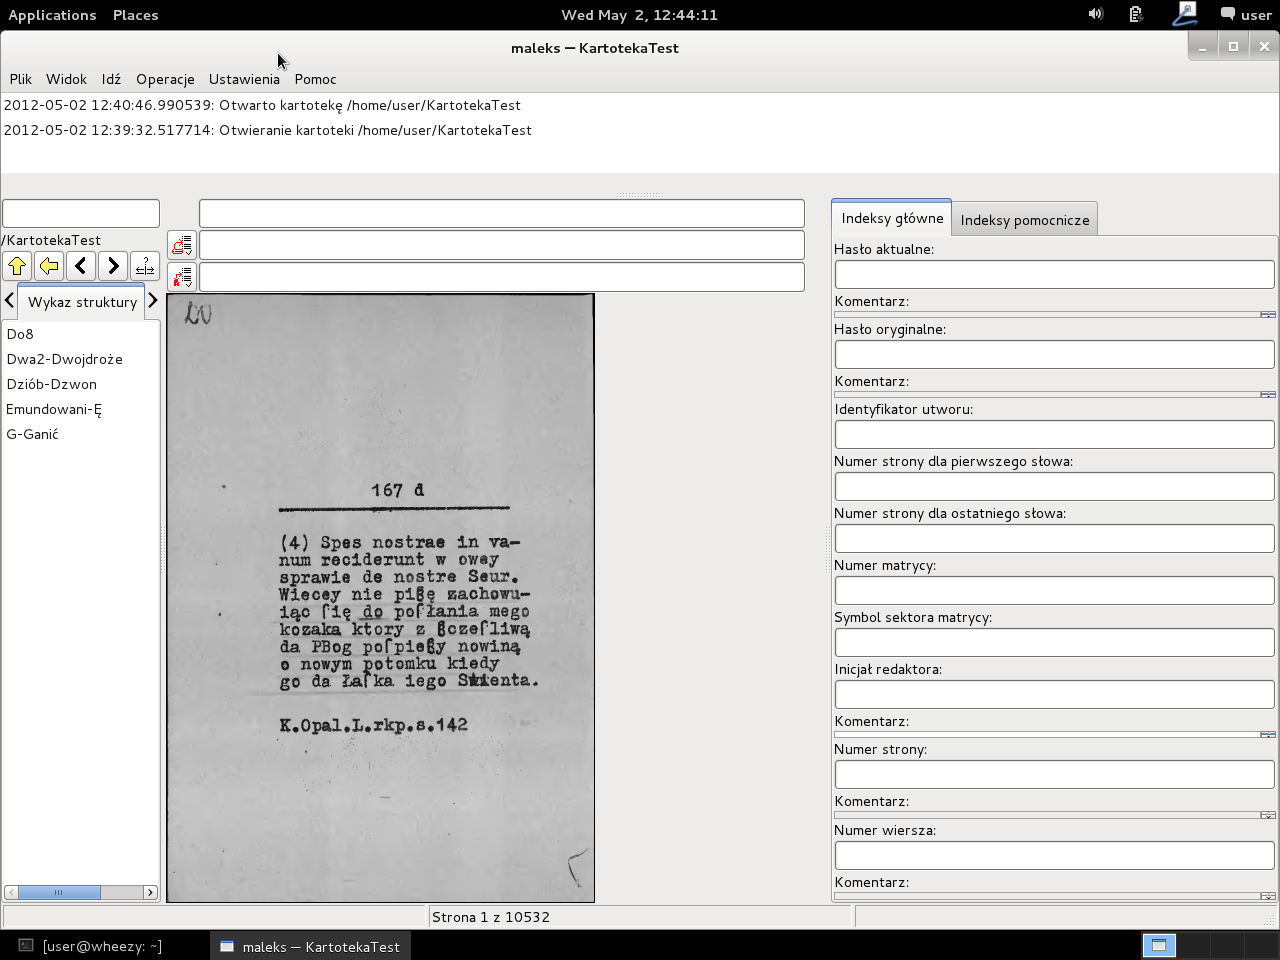
\includegraphics[scale=0.3]{02_otwartabaza.png}

Program dąży do znalezienia pierwszej i ostatniej fiszki w poszukiwanym przez nas zakresie. Dlatego też stara się zlikwidować tworzące się w toku indeksowania luki na liście haseł. Jednocześnie wyświetla informację, ile fiszek znajduje się w danej luce. Podczas indeksowania program celuje więc w to miejsce, w którym zgodnie z układem alfabetycznym powinna znajdować się odpowiednio pierwsza i ostatnia poszukiwana fiszka.  

%Po zaindeksowaniu dwóch fiszek na liście haseł tworzy się luka z informacją, ile fiszek się tam znajduje. Kiedy ponownie szukamy swojego hasła, program celuje w tę lukę, w której zgodnie z układem alfabetycznym powinna znajdować się fiszka. 

Indeksujemy kolejne fiszki aż do momentu, w którym program w polu komunikatów poinformuje, że wyszukiwanie zostało zakończone i ile kroków to wymagało (por. rys. \ref{09episkop_koniec} na s. \pageref{09episkop_koniec}).


\begin{figure}[h]
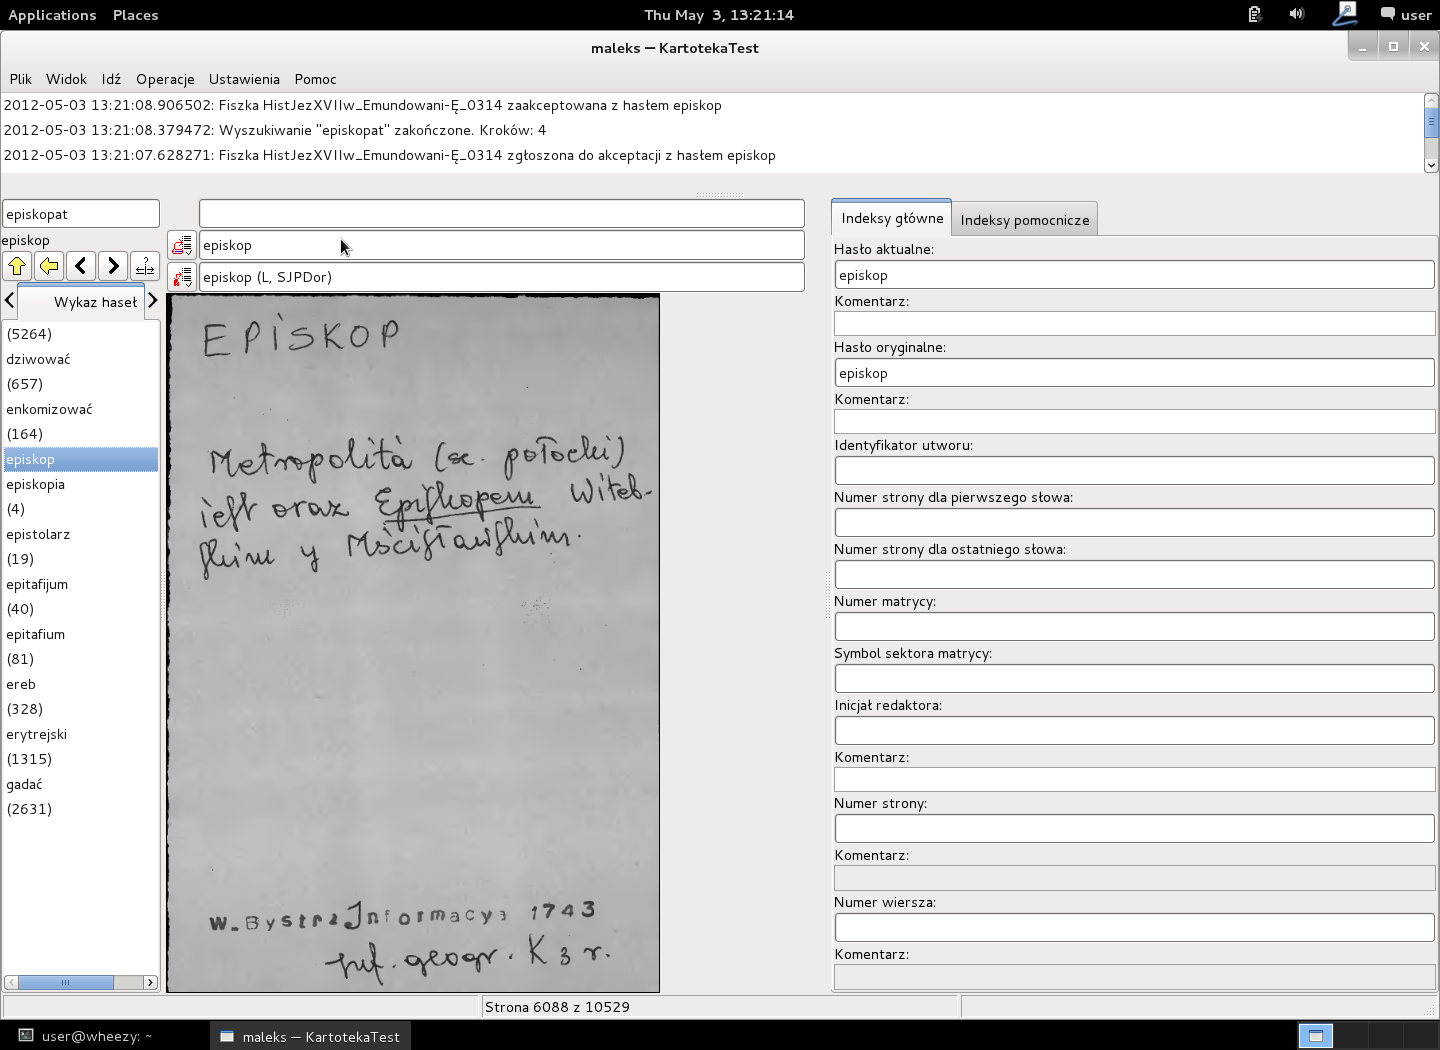
\includegraphics[scale=0.3]{09episkop_koniec.png}
\caption{Koniec wyszukiwania}
\label{09episkop_koniec}
\end{figure}

\begin{figure}[h]
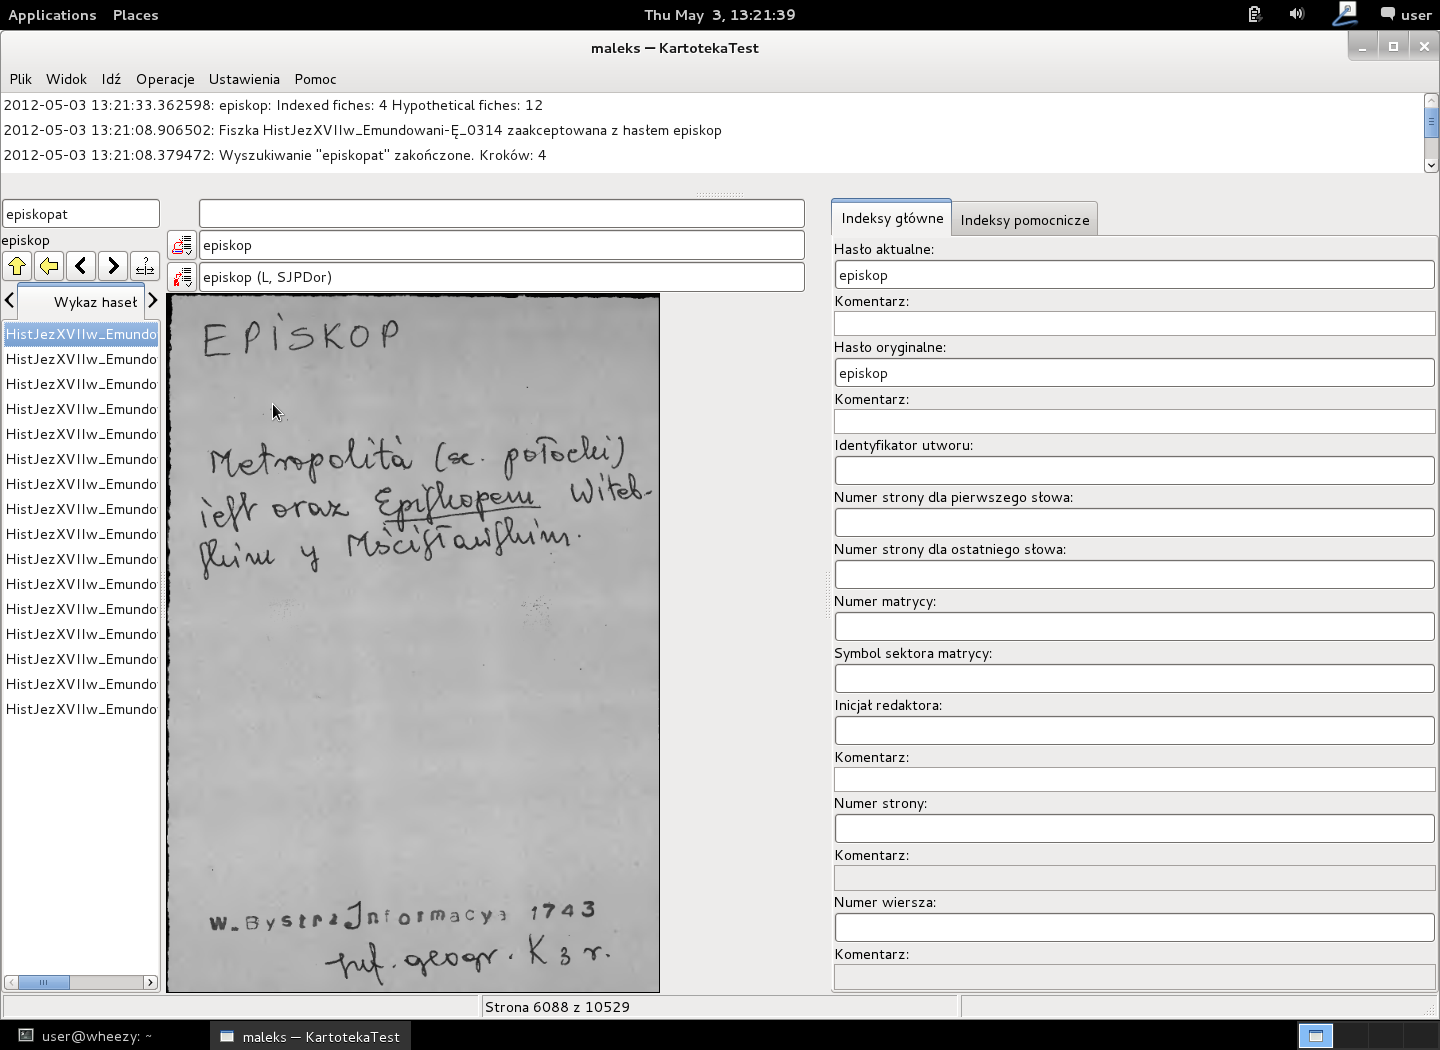
\includegraphics[scale=0.3]{10doindeksowanie.png}
\caption{Doindeksowywanie hipotetycznych fiszek}
\label{10doindeksowanie}
\end{figure}


W tym momencie mamy wyekscerpowaną grupę fiszek, z których co najmniej pierwsza i ostatnia są zaindeksowane jako fiszki odpowiadające poszukiwanemu hasłu. Należy więc wejść do podglądu tego przedziału fiszek (za pomocą skrótu \texttt{Ctrl+Enter}), obejrzeć skany, sprawdzić, czy zostały dobrze wskazane jako odpowiadające kwerendzie i zaindeksować je ręcznie (por. rys. \ref{10doindeksowanie} na s. \pageref{10doindeksowanie}).

\begin{figure}[h]
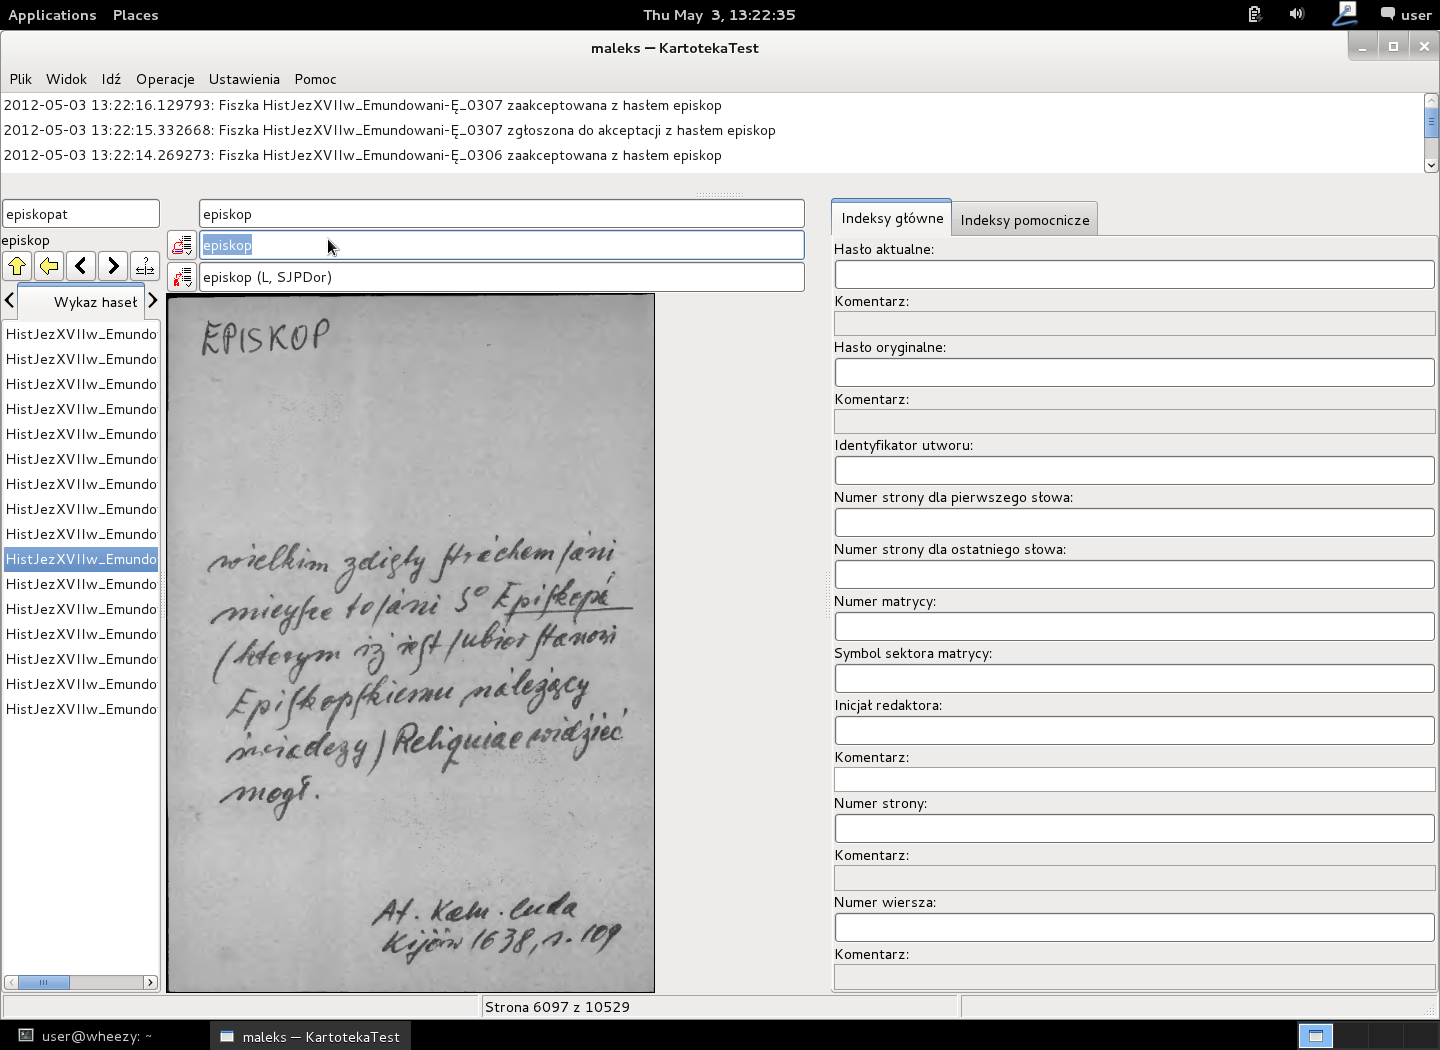
\includegraphics[scale=0.3]{11episkop_zpodpowiedzi.png}
\caption{Fiszka z hasłem w polu hipotez}
\end{figure}

\begin{figure}[h]
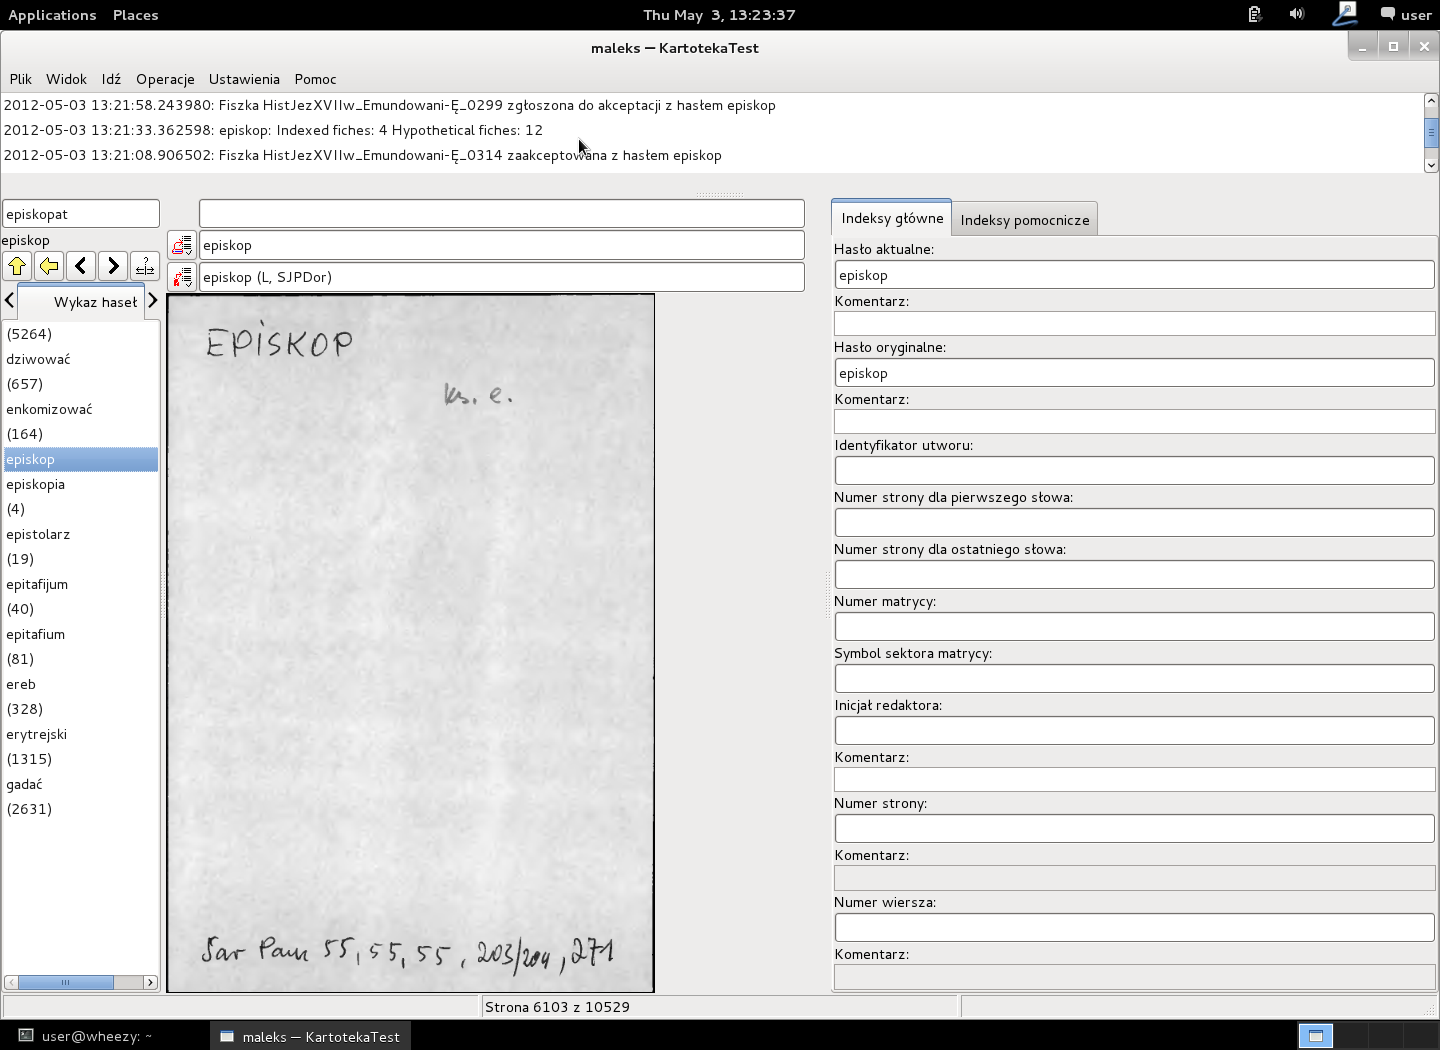
\includegraphics[scale=0.3]{12episkop_hipotetycznefiszki.png}
\caption{Hipotetyczne fiszki}
\label{hipotetyczne}
\end{figure}


%\section{Aktualizacja}
%
%W terminalu w katalogu \texttt{/home/user/maleks} wpisujemy polecenia:
%
%\texttt{hg pull --update}
%
%\texttt{su} (i podajemy hasło)
%
%\texttt{python setup.py install}

\section{Lista skrótów}


\texttt{Ctrl+Enter} --- rozpoczyna kwerendę w polu kwerend

\texttt{Ctrl+B} --- wyłącza/przywraca wyszukiwanie binarne w polu kwerend

\texttt{Ctrl+H} --- akceptuje podpowiedzi z innych słowników i zapisuje je w polu edycji

\texttt{Ctrl+strzałka} --- wyszukuje w polu edycji hasła z historii

\texttt{Enter} --- akceptuje hasło z pola edycji

\texttt{Ctrl+V} --- wyświetla podgląd fiszek

\texttt{strzałka góra/dół} --- nawigacja w podglądzie fiszek

\texttt{Ctrl+K} --- klonowanie fiszek (nie działa w trybie wyszukiwania binarnego)

\texttt{Ctrl+D} --- dodanie zakładki do fiszki

Pełna lista jest dostępna w samym programie w części menu o nazwie \texttt{O programie} (por. rys. \ref{skroty} na s. \pageref{skroty}) oraz w manpage'ach programu. 

\begin{figure}[h]
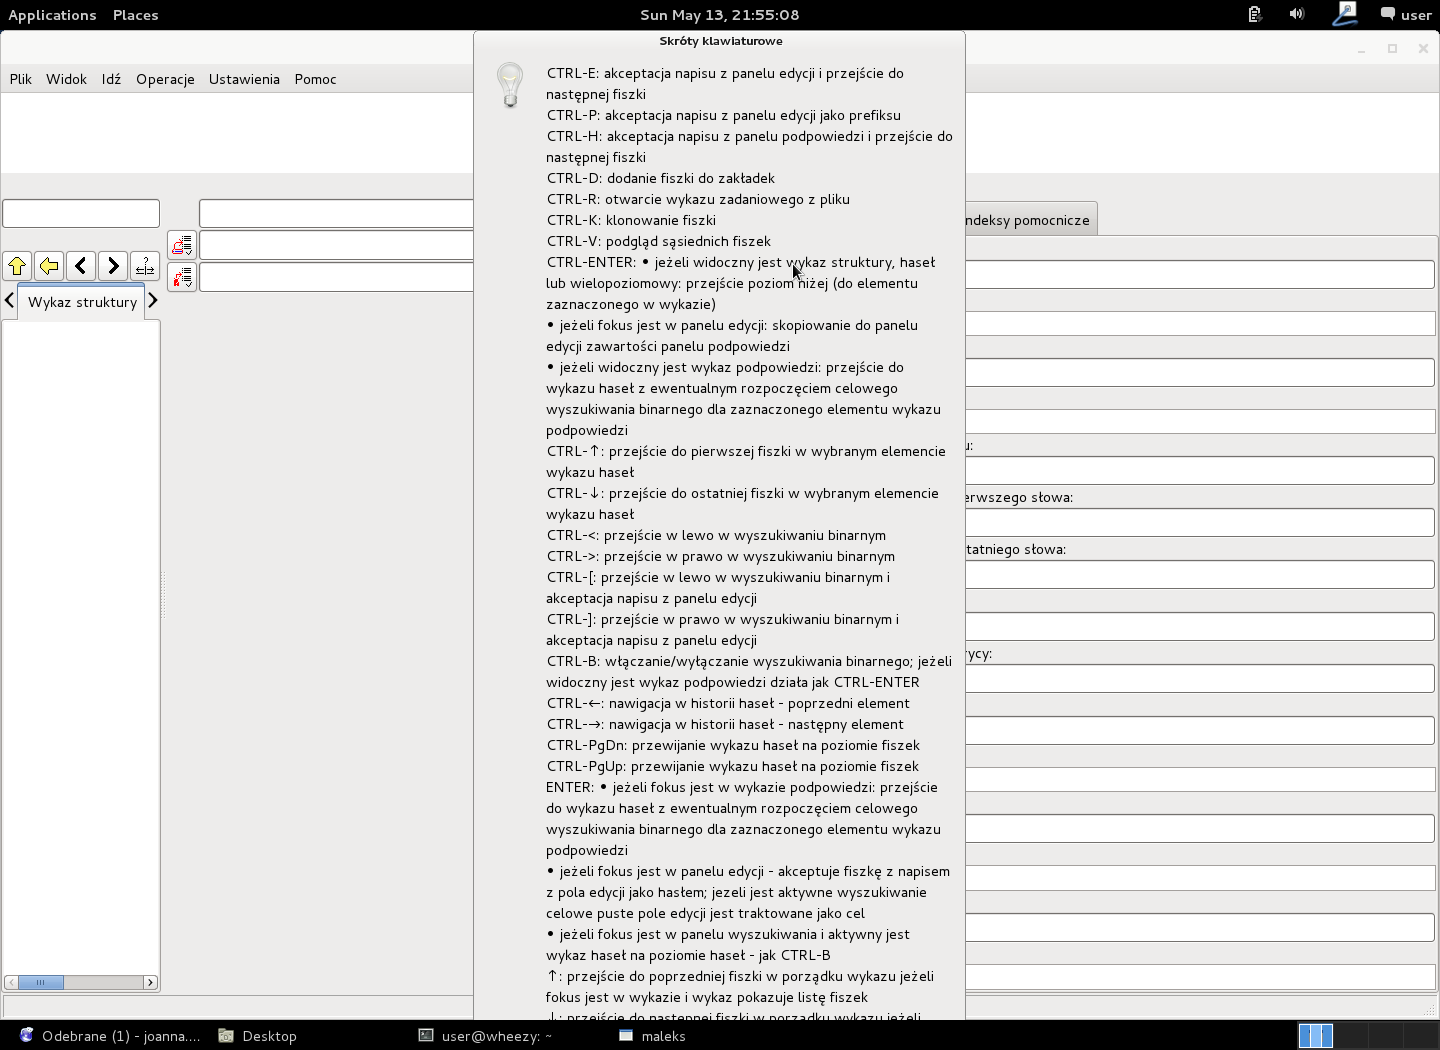
\includegraphics[scale=0.3]{skroty2.png}
\caption{Fragment listy skrótów}
\label{skroty}
\end{figure}

\thebibliography{2012}
\bibitem{bien2012}Janusz S. Bień, \textit{Dygitalizacja kartotek słownikowych} (w druku), \url{http://bc.klf.uw.edu.pl/256/}.

\bibitem{ndt}Witryna grantu MNiSzW nr NN519 384036, \url{https://bitbucket.org/jsbien/ndt}.

\bibitem{sxvii}Witryna \textit{Słownika języka polskiego XVII i 1. połowy XVIII wieku}, \url{http://sxvii.pl}.

\bibitem{maleks}Witryna przeglądarki materiałów leksykograficznych \texttt{maleks}, \url{https://bitbucket.org/tomek87/maleks}.


\end{document}